\subsection{Storage Space and Impact on Fault Tolerance}
 
\begin{figure}
    \centering
    \subfigure[Sharing of data under VM-centric dedup model]
    {
        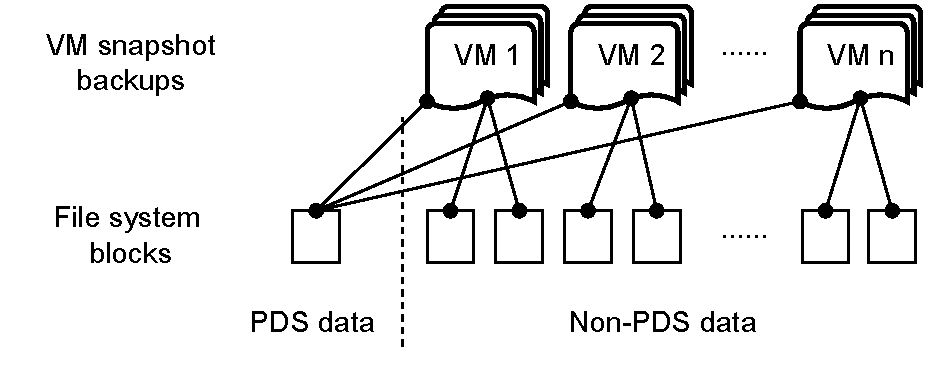
\includegraphics[width=3in]{images/share_vc}
        \label{fig:share_vc}
    }
    \\
    \subfigure[Sharing of data under VM-oblivious dedup model]
    {
        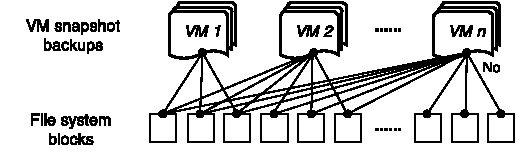
\includegraphics[width=3in]{images/share_vo}
        \label{fig:share_vo}
    }
    \caption{Bipartite association of VMs and file blocks under VO and VC approaches}
    \label{fig:share}
\end{figure}

The replication degree of the backup storage 
is $r$ for regular file blocks and $r=3$ is a typical setting in the distributed
file system~\cite{Hadoop,GFS}.
In the VC approach, a special replica degree $r_c$ used for PDS blocks where $r_c>r$. 
The storage cost for VO with full deduplication is $c_u *r$ and for VC, it is
$ k*r_c  + (c_u-k)*r$. Thus The storage cost ratio of $VC$ over $VO$ is 
\[
\sigma \frac{r_c}{r} + 1-\sigma
\]
Since $sigma$ is small,  term $\sigma \frac{r_c}{r}$ is small in the above expression.  
Thus the impact on storage increase is very small when we choose a large $\frac{r_c}{r}$ ratio. 
For example, $\frac{r_c}{r}=2$. 


%In our experiment with Alibaba data, the ratio $\sigma$ 
%is 162. Thus allocation of extra replicas for PDS only introduces a small amount of extra space
%cost.  Figure~\ref{fig:storagePDS} shows the storage cost ratio of VC and VO when 
%$r$=3, and $r_c$ varies from 3 to 10.
%The result shows that the storage cost for adding extra replication for PDS
%is insignificant.

Next we  assess  the impact of losing $d$ machines 
to the the VC and VO approaches.  
A large $\frac{r_c}{r}$ ratio can have a positive impact on full availability of snapshot blocks.


\comments{
For each rank $i$ block which appears $C_i$ times  among $V$ virtual machines.
Assigning this block to virtual machines can be viewed as a classical ball-bin assignment
approximated by a Poisson distribution. Namely the virtual machines that share this block
is approximated as $1 -  e^{C_i/V}$.
Thus the average number of VMs that share a block is:
\[
(1-\delta) + \delta \sum_1^{u_b} \frac{1 -  e^{C_i/V}}{u_b}.
\]
Any failure of a block would impact the above number of virtual machines.
In VO, the number of VMs that share a block is:
\[
\sum_1^{u_b'} \frac{1 -  e^{C_i'/V}}{u_b'}.
\]

Next we discuss how a failure of $d$ machines impacts the VM snapshots in VC.
When $d<r$, there is no loss of data in the snapshot storage.
When $r_c> d \ge r$, some of data blocks in the storage are lost, and we compute the number of VMs that could
suffer the loss of their snapshots.
When $d \ge r_c$, some of PDS blocks are affected.
In VC, the blocks in PDS are stored in a container manner (superblock), and they are shared by many VMs.
The number of data containers stored with replication degree $r$ for
referenced by each VM is:
\[
N_1= \frac{b}{v*s} (1-\delta) +b/(v*s)\delta (1 -  (\frac{k}{b_u})^{1-\alpha}).
\]
The number of PDS data containers stored with replication degree $r_c$ for
referenced by each VM is:
\[
N_2= \frac{b}{v*s}\delta (\frac{k}{b_u})^{1-\alpha}.
\]
}



%Thus the number of VMs using a block =    $(1-s_c)  + s_c *L$.
%In characterizing the reliability of VM backups in our model, 
%we consider the likely hood that a file system block fails,
%given some number of storage machine failures. 
%Every time a filesystem block fails,
%we say that we have lost data for that virtual machine, so it is no longer
%available. 
%In reality it may be only one snapshot that is affected, but it is the user
%who must decide which snapshots are important, so we consider the worst case. 
We use filesystem blocks rather than a deduplication
data chunk as our unit of failure because the DFS keeps
filesystem blocks as its base unit of storage.
% (in our case there are 
%16384 blocks in a filesytem block on average, with 4KB block size and 
%a 64MB block size).
To  compute the full availability of all snapshots of a VM, we derive
the probablity of losing a snapshot file block of a VM by
estimating the number of file system blocks per VM in each approach.
As illustrated in Figure~\ref{fig:share},
we build a bipartite graph representing the association from unique file system blocks
to their corresponding VMs in each approach. An association edge is  drawn  from a file block  to a VM 
if this block is used by this VM. 
For VC, each VM has an 
average number of $N_1$ file system blocks for non-PDS data. 
It also refers  an average of   $N_2$ file system blocks for PDS data. 
For VO, each VM has an average  of  $N_o$ file system blocks
and let $V_o$ be the average number of VMs shared by each file system block.
%Figure~\ref{fig:shared} illustates the bipartite association.

In VC, each non-PDS file system block is associated with one VM
 and  PDS file system blocks are
shared by an average of $V_c$ VMs. Let $s$ be the average number of chunks per file block. Thus, 
\[
V *p*N_1 *s  = C_u (1-\sigma)\; \mbox{ and } \; 
V *p*N_2 *s  = C_u \sigma *V_c
\]
For the VO approach, 
\[
V *p*N_o *s  = C_u  V_o.
\]

Since each file block (with default size $64MB$) contains many chunks (on average 4KB),
each file block contains the hot low-level chunks shared by many VMs, and it also contains
rare chunks which are not shared.  From the about equations.
\[
\frac{N_1}{N_o}=  \frac{1-\sigma}{V_o}<1.
\] 
Thus when there is a failure in file blocks with replication degree $r$
and there is no failure for PDS data with more replicas,   a VM in
the VC approach has a lower chance to lose a snapshot than the VO approach because
$N_1<N_o$. 
Figure~\ref{fig:fsb-links} shows the number of VMs sharing by each file block.
%In our experiment, we find that $V_o \approx 0.2 V$ when backing up VMs one by one.
We can observe that $N_1 +N_2 < N_o$. 
This is likely because the PDS FSBs tightly pack data used by many VMs, 
which decreases the overall number of FSBs required to backup a VM.
If  the backup for multiple VMs is conducted concurrently, there would be more
VMs shared  by each file block on average. Therefore,
even when there is a loss of a PDS block, the VC approach tolerates the fault better.

%Figure~\ref{fig:fsb-links} shows the average number of VMs sharing a
%filesystem block (FSB) as VMs are added. Though we don't expect the linear trend to continue indefinitely for
%much larger datasets, it should continue to increase, which has important implications
%on VM backup availability in the precense of failures. Below we show the
%significant impact the number of links has on VM backup reliability.

\comments{%dropping block links bec. we don't use it elsewhere
\begin{figure}[htbp]
  \centering
  %\includegraphics[scale=.45,natwidth=511,natheight=276]{vo_links}
	\begin{tikzpicture}
		\begin{axis}[
		%title={VO Block links},
		xlabel={Number of VMs added},
		ylabel={Avg. links to a chunk},
		%extra y ticks={4.5,5.5,6.5} %because it only shows 4,5,6,7
		legend pos=south east
		]
		\addplot table[x=VMs,y=Measured] {figures/vo_links.txt};
		\addplot table[x=VMs,y=Theoretical] {figures/vo_links.txt};
		\legend{Measured,Theoretical};
		\end{axis}
	\end{tikzpicture}
  \caption{Average number of VMs sharing a data chunk in the global index}
  \label{fig:vo-links}
\end{figure}
}

\begin{figure}[htbp]
  \centering
	\begin{tikzpicture}
		\begin{axis}[
                width=\linewidth,
                height=0.6\linewidth,
		%title={VO FSB links},
		xlabel={Number of VMs},
		ylabel={Avg. Num. VMs sharing FSB},
                cycle list name=mline,
                xmin=0,
                ymin=0,
                xmax=106,
		%extra y ticks={4.5,5.5,6.5} %to show extra ticks
		legend pos=north west
		]
                \addplot table[x=VMs,y=FSBLinks] {figures/vo_fsb_links_105.txt};
		\addplot table[x=VMs,y=cdslinks] {figures/cds_links_105.txt};
                \legend{VO, PDS in VC};
		\end{axis}
	\end{tikzpicture}
  \caption{Measured Average number of VMs sharing a 64MB FSB with global dedup (VO), and in a 2\% PDS for VC.}
  \label{fig:fsb-links}
\end{figure}



\begin{figure}[htbp]
  \centering
	\begin{tikzpicture}
		\begin{axis}[
		%title={VO VM links},
                width=\linewidth,
                height=0.6\linewidth,
		xlabel={Number of VMs},
		ylabel={Avg. Num. FSBs used by VM},
                xmin=0,
                ymin=0,
                xmax=106,
		%extra y ticks={4.5,5.5,6.5} %to show extra ticks
		legend pos=south west
		]
                \addplot[blue,mark=none] table[x=VMs,y=No] {figures/vo_vm_links_105.txt};
                \addplot[red,dotted,mark=none] table[x=VMs,y expr=\thisrow{N1}+\thisrow{N2}] {figures/vc_vm_links_105.txt};
                \addplot[red,dashdotted] table[x=VMs,y=N1] {figures/vc_vm_links_105.txt};
                \addplot[red,densely dashed,mark=none] table[x=VMs,y=N2] {figures/vc_vm_links_105.txt};
                \legend{$N_o$, $N_1+N_2$, $N_1$, $N_2$};
		\end{axis}
	\end{tikzpicture}
  \caption{Measured Average number of 64MB FSBs used by a single VM. For VC both the number of PDS and Non-PDS FSBs used are shown.}
  \label{fig:vm-links}
\end{figure}


 The full snapshot availability of a VM is estimated as follows with parameters $N_1$, $N_2$, and $N_o$.
%the likelyhood that there is no  data loss for all its file blocks.  
With replication degree $r$, the availability of a file block is the probability that  
all of its replicas do not appear in any group of $d$ failed machines. 
Namely, $1-\binom{d}{r}/ \binom{p}{r}$. 
The snapshot availability of a VM  in the VO approach is
\begin{equation}
\label{eq:VO}
(1-\frac{ \binom{d}{r}} { \binom{p}{r} })^{N_o}. 
\end{equation}

%This can be seen in Figure~\ref{fig:fsb-availability} for a 100 machine cluster for 3 different replication factors.
For VC, there are two cases.
\begin{itemize}
\item
When there are $r \le d<r_c$ machines failed,  there is no PDS data loss and  
%a file block failure depends on if all replicas of this container reside in the failed machines.
the full snapshot availability of a VM in the VC approach is 
and is
\[
(1-\frac{\binom{d}{r}} { \binom{p}{r} })^{N_1}.
\]
%\begin{multline}
%= Probability (\mbox{ There is no file block loss in this VM}) \\
%= Probability(\mbox{ A file block has file data loss})^{N_1}\\
%= (1- Probability (\mbox{all replicas of its block fail}))^{N_1}\\
%\end{multline}
%\end{split}
Since $N_1 <N_o$, the VC approach has a higher availability of VM snapshots than VO.

\item
When $r_c \leq d$, both non-PDS and PDS file blocks in VC can have a loss.
The full snapshot availability of  a VM in the VC approach is
\[
(1-\frac{ \binom{d}{r}} { \binom{p}{r} })^{N_1} 
*
(1-\frac{ \binom{d}{r_c}} { \binom{p}{r_c} })^{N_2}.
\]
Figure~\ref{fig:fsb-availability} illustrates that the availability of an individual file system block
with different replication degree. This demonstrates inequality $1-\frac{ \binom{d}{r}} { \binom{p}{r} }
< 1-\frac{ \binom{d}{r_c}} { \binom{p}{r_c} }$. As we have also observed
$N_1+N_2 <N_o$ in our dataset, these two conditions support that VC has a  higher availability. 
%comparing  Formula~\ref{eq:VO} and~\ref{eq:VC}. 
\end{itemize} 

%= Probability(\mbox{ No non-PDS file block loss})^{N_1}
%Probability(\mbox{ No PDS file block loss})^{N_2}\\
%\begin{multline}
%\end{split}
%\end{multline}




%By comparison, the probability that a VM has data loss is close to
%1 once  there are  $d \ge r$ failed machines. That is because there are more data blocks
%shared among VMs. Any failure of these blocks causes many more VMs to fail.


\comments{
We take the likelyhood of VM failure to be the same as the likelyhood of chunk failure,
so
\[
    P_{VMfailure}=\frac{\binom{d}{r}}{\binom{p}{r}}
\]

Since both in the PDS and in the VO approach a single filesystem chunk may be used by many VMs,
we must multiply the block failure ratio by the number of outgoing links for the block to get
the expected impact on the system.
\[
    E_{VMfailure}=L\frac{\binom{d}{r}}{\binom{p}{r}}
\]

in our current testbed we have measured the average number of links per chunk
(Figure~\ref{vo-links}) and number of links per Filesystem Block (FSB)
(Figure~\ref{fig:fsb-links}) in our dataset. For the complete dataset, we also
found the average number of links to PDS chunks, which was \~19 using a 2\%
PDS. From Figure~\ref{fig:fsb-links} you can see that as you add VMs, the
average number of links to a chunk increases linearly for our dataset. We
expect that this trend will level out with larger datasets, but should continue
to increase at a slower rate.  For the VC model, we have to consider both PDS
chunks and non-PDS chunks. In the VO model all data is shared, but in VC only
the PDS data is shared, but at a much higher rate. This gives a strong
advantage to VC, in that for a large percent of the data (95-99\%), there is
only one VM pointing to each non-PDS chunk. You can see the increase in
reliability in Figure~\ref{fig:vm-availability}.
\begin{table}
    \begin{tabular}{|l|lll|}
    \hline
    \multirow{2}{*}{Nodes Failed}   & \multicolumn{3}{c|}{Availability(\%)}\\
                                    & $R=3$ & $R=4$ & $R=5$\\
    \hline
    1           &  100      & 100       & 100\\
    2           & 100       & 100       & 100\\
    3          & 99.999     & 100       & 100\\
    5          & 99.993     & 99.9999   & 99.999998\\
    10          & 99.926    & 99.995    & 99.999\\
    20          & 99.295    & 99.876    & 99.979\\
    \hline
    \end{tabular}
    \caption{Availability in a 100 machine cluster of a single FSB with different replication factors}
    \label{tab:fsb-availability}
\end{table}

}

\begin{figure}[htbp]
  \centering
    \begin{tikzpicture}
            \begin{axis}[
                width=\linewidth,
                height=0.6\linewidth,
            %title={FSB Availability},
            cycle list name=mline,
            xlabel={Number of Machines Failed},
            ylabel={Availability of Single FSB (\%)},
            extra y ticks={99.9}, %to add extra ticks
            mark options=solid,
            legend pos=south west,
            %legend columns=2,
            %legend style={
            %    at={(0.5,-0.2)},
            %anchor=north}
            ]
            \addplot table[x=NodesFailed,y=Availability5] {figures/fsb_availability.txt};
            \addplot table[x=NodesFailed,y=Availability4] {figures/fsb_availability.txt};
            \addplot table[x=NodesFailed,y=Availability3] {figures/fsb_availability.txt};
            \legend{$R=5$,$R=4$,$R=3$};
            \end{axis}
    \end{tikzpicture}
    \caption{Availability of individual file system blocks in a 100 machine cluster with different replication degrees.}
  \label{fig:fsb-availability}
\end{figure}





